\section{Introduction}
\label{sec.intro}

Debugging bug reports, which often come in a high volume~\cite{AnvikHM05}, has proved to be a difficult task that consumes much resources and time~\cite{tassey02economic}. Various techniques have thus been devised to help developers locate buggy program elements from their symptoms. These symptoms could be in the form of a descriptions of a bug experienced by a user, or a failing test case. These techniques, often collectively referred to as bug (or fault) localization, would analyze the symptoms of a bug and produce a list of program elements ranked based on their likelihood to contain the bug.

Existing bug localization techniques broadly fall into two major categories: \emph{information retrieval} (IR)-based techniques~\cite{Rao:2011:RSL:1985441.1985451,Sisman:2012:IVH:2664446.2664454,Zhou:2012:BFM:2337223.2337226,SahaLKP13}, and \emph{spectrum}-based bug localization techniques~\cite{JH05,Abreu:2009,RR03,ZH02,Zeller2002a,CZ05,LAZJ03,Libl+05,LYFHM05}. The IR-based bug localization techniques typically analyze textual descriptions contained in bug reports and identifier names and comments in source code files. They then return a ranked list of program elements (typically program files) that are the most similar to the bug textual description. The spectrum-based bug localization techniques typically analyze program spectra that corresponds to program elements that are executed by failing and successful execution traces. Likewise, they return a ranked list of program elements (typically program blocks or statements) that are executed more often in the failing rather than correct traces.

% What are the latest trend
% Why multi-modal bug localization make sense?

The above-mentioned approaches, however, only consider one kind of symptom or one source of information, i.e., only bug reports or only execution traces. This is a limiting factor since hints of the location of a bug may be spread in both bug report and execution traces; and some hints may only appear in one but not the other. In this work, we put forward a bug localization approach that addresses the deficiency of existing methods by jointly utilizing both bug reports and execution traces. We refer to this approach as {\em multi-modal bug localization}, as we need to consider multiple modes of inputs (i.e., bug reports and program spectra). Such an approach fits well to developers' debugging activities as illustrated by the following scenarios:

\begin{enumerate}
	\item Developer $D$ is working on a bug report that is submitted to Bugzilla. One of the first tasks that he needs to do is to replicate the bug based on the description in the report. If the bug can be successfully replicated, he will proceed to the debugging step; otherwise, he will mark the bug report as ``WORKSFORME'' and will not continue further~\cite{worksforme}. After $D$ replicates the bug, he has one or a few failing execution traces. He also has a set of regression tests that he can run to get successful execution traces. Thus, after the replication process, $D$ has {\em both} the textual description of the bug and a program spectra that characterizes the bug. With this, $D$ can proceed to use multi-modal bug localization.
	\item  Developer $D$ runs a regression test suite and some test cases fail. Based on his experience, $D$ has some idea why the test cases fail. $D$ can create a textual document describing the bug. At the end of this step, $D$ has {\em both} program spectra and textual bug description, and can proceed to use multi-modal bug localization which will leverage not only the program spectra but also $D$'s domain knowledge to locate the bug.
\end{enumerate}

% Although no multi-modal bug localization technique has been proposed in the literature, there are a few multi-modal feature location techniques. These techniques process both feature description and program spectra to recommend program elements (typically program methods) that implement a corresponding feature~\cite{PoshyvanykGMAR07,LiuMPR07,DitRP13}. These feature location approaches can be adapted to locate buggy program elements by replacing feature descriptions with bug reports and feature spectra with buggy program spectra. Unfortunately, our experiment (see Section~\ref{sec.exp}) shows that the performance of such adapted approaches are not optimal yet.

\begin{figure*}[!t]
	\centering
	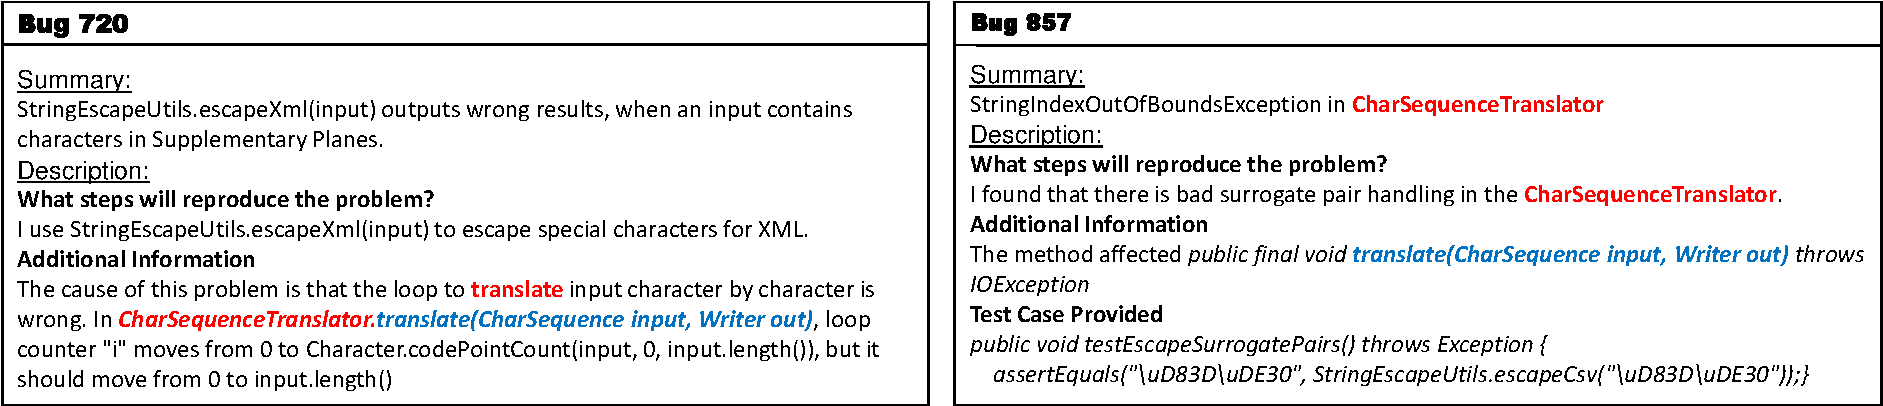
\includegraphics[width=\textwidth]{bug_example.pdf}
	\caption{Example of two bug reports which have same faulty method in project Lang}
	\label{fig:bug_motivation}
\end{figure*}

It is worth noting that our work focuses on localizing a bug to the \emph{method} that contains it. Historically, most IR-based bug localization techniques aim at finding buggy files~\cite{Rao:2011:RSL:1985441.1985451,Sisman:2012:IVH:2664446.2664454,Zhou:2012:BFM:2337223.2337226,SahaLKP13}, while most spectrum-based techniques find buggy lines~\cite{JH05,Abreu:2009,RR03}. Although it is useful to localize a bug to the file that contains it, the file size can be big and developers still need to go through a lot of code to find the few lines that contain the bug. On the other hand, while localizing a bug to the line that contains it is also useful, a bug often spans across multiple lines. Furthermore, developers often do not have ``perfect bug understanding''~\cite{ParninO11} and thus by just looking at a line of code, developers often cannot determine whether it is the location of the bug and/or understand the bug well enough to fix it. Localization at the method level presents a good tradeoff; a method is not as big as a file, but it often contains sufficient context needed to help developers understand a bug.

%Poshyvanyk et al. proposed an approach named PROMESIR that computes weighted sums of scores returned by an IR-based feature location solution and a spectrum-based feature location solution, and ranks program elements based on these scores~\cite{PoshyvanykGMAR07}. Liu et al. proposed an approach named SITIR which filters program elements returned by an IR-based feature location solution if they are not executed in a failing execution trace~\cite{LiuMPR07}. Dit et al. use HITS, a popular algorithm that ranks the importance of nodes in a graph, to filter program elements returned by SITIR~\cite{DitRP13}. Their paper highlights two best performing variants that outperform SITIR, which differ on how the graph to be analyzed by HITS is generated; we refer to these variants as $DIT^{A}$ and $DIT^{B}$ in this paper.

% How our approach might help ? Why the approach would work ? Intuition. Cite Parnin and Orso's work here.
% Our multi-modal bug localization approach improves previous multi-modal approaches based on two intuitions. First, we note that there are a wide variety of bugs~\cite{ThungWLJ12,XiaZLZ13} and different bugs often require different treatments. Thus, there is a need for a bug localization technique that is adaptive to different types of bugs. Past approaches~\cite{LiuMPR07,DitRP13,PoshyvanykGMAR07} propose a one-size-fits-all solution. Here, we propose an instance-specific solution that considers each bug individually and tunes various parameters based on the characteristic of the bug. Second, Parnin and Orso~\cite{ParninO11} highlight in their study that some words are useful in localizing bugs and suggest that ``future research could also investigate ways to automatically suggest or highlight terms that might be related to a failure''. Based on their observation, we design an approach that can automatically highlight {\em suspicious words} and use them to localize bugs.



In this paper, we present a new approach called the \underline{Net}work-clustered \underline{M}ulti-modal Bug \underline{L}ocalization (NetML), which works based on three main intuitions. Firstly, it is established that a wide variety of bugs exist~\cite{ThungWLJ12,XiaZLZ13}, and different bugs often require different treatments. Hence, there is a need to have separate latent parameters for different bugs, which are tailored to the characteristics of the individual bugs. Similarly, different program elements (or methods in this work) are of different nature, and should be characterized using separate latent parameters. Secondly, Parnin and Orso~\cite{ParninO11} found in their studies that some words are more useful in localizing bugs, and suggested that ``future research could also investigate ways to automatically suggest or highlight terms that might be related to a failure''. NetML provides such capability by incorporating \emph{method suspiciousness} feature, which allows us to automatically highlight suspicious terms and use them to localize bugs. Lastly, we recognize that bugs and program elements are \emph{not} completely independent, and some bugs (or methods) may be more similar to certain bugs (or methods) than to others. As such, similar bugs (or methods) should have latent parameters that are close together, which can then be exploited to localize bugs more effectively. 

Figure~\ref{fig:bug_motivation} presents an example of two bug reports which motivate our intuitions. Bug 720 has an ``outputs wrong results'' error when an input contains ``characters in \textit{Supplementary Planes}'' whereas Bug 857 contains ``\textit{StringIndexOutOfBoundsException}'' error. These two bugs ultimately reside in the \texttt{translate} method in the \texttt{CharSequenceTranslator.java} program. Based on text descriptions, these two bugs are quite independently since they provide two different bugs in Lang. However, Bug 720 and Bug 857 should be similar since they share the same \texttt{translate} method and \texttt{CharSequenceTranslator.java} program. At a text level space, we are unable to capture the similarity between two bug reports. 

Some of these intuitions have already been captured in our recent work---dubbed \underline{A}daptive \underline{M}ulti-Modal Bug \underline{L}ocalization (AML)~\cite{Le:2015:IRS:2786805.2786880}--- which we extend in this journal paper. In particular, AML already incorporates the ideas of adaptively computing separate latent parameters for each bug report, and of computing the method suspiciousness score.
%where we proposed \underline{A}daptive \underline{M}ulti-modal bug \underline{L}ocalization (i.e., AML) consisting of three different components:  AML$^\text{Text}$, AML$^\text{Spectra}$, and AML$^\text{SuspWord}$. AML$^\text{Text}$ only considers the textual description in bug reports, and AML$^\text{Spectra}$ only considers program spectra. On the other hand, AML$^\text{SuspWord}$ takes into account suspicious words learned by analyzing textual description and program spectra together. Typically, AML$^\text{SuspWord}$ computes the {\em suspicious scores} of words that appear as comments or identifiers of various program elements. It associates a program element to a set of words and the suspiciousness of a word can then be computed based on the number of times the corresponding program elements appear in failing or correct execution traces. Each of these components would output a score for each program element, and AML computes the weighted sum of these scores by forcing all program elements to share the same tuple of component weights ($\alpha, \beta, \gamma$) which corresponds to AML$^\text{Text}$, AML$^\text{Spectra}$, and AML$^\text{SuspWord}$, respectively. 
%. The final score is {\em adaptively} computed for each individual bug by tuning these weights. 
However, the current AML approach exhibits two main shortcomings. Firstly, AML only has the concept of latent parameters for bug reports, but not for program elements (or methods). As such, it is not able to capture the variation in the (latent) characteristics of different program elements (methods), which may limit its effectiveness in localizing a bug. Secondly, the latent parameters of each bug report are learned independently of those of other bug reports. As a result, AML is unable to take advantage of the clustering/similarity traits of different bug reports in the localization process.

%\begin{itemize}
%	\item First, the final suspiciousness score only assumed that all the program elements share the same parameter vector of bug report. In practice, each program element not only considers the parameter vector of bug reports but also share the parameter of program elements. For example, we call $f_{ij}$ as the suspiciousness score of program element $i$ related to bug $j$, and $sim_{ij}$ measures the similarity between program element $m_i$ and $m_j$. Assuming that our dataset only includes three program elements which are $m_1$, $m_2$, $m_3$ and one bug report $b_1$, and their suspiciousness score results are ranked as $f_{11} > f_{21} > f_{31}$. Moreover, we also assume that 
	%the program element $m_1$ and $m_3$ have a high similarity score compared to $m_2$. In other words, %
	%the similarity scores of $m_1$, $m_2$ and $m_3$ are expressed as following ($sim_{13} \gg sim_{12}$) and ($sim_{13} \gg sim_{23}$). According to the suspiciousness score ranking, $m_1$ has highly related to bug report $b_1$. Furthermore, $m_1$ and $m_2$ have a high similarity score compared to $m_2$, and hence our suspiciousness ranking should be $(f_{11} \approx f_{31}) > f_{21}$. However, AML only assumes that each program element shares the same weight vector of bug report without considering its distinctive functionalities and properties, leading to the suspiciousness ranking score of AML may be inaccurate. 
	%rank of similarity scores between different program elements are presented as ($sim_{13} \gg sim_{12}$)
	%\item Second, the parameter vector of bug report $b$ is learned independently of other bug reports, without exploiting the clustering and/or similarity properties of different bug reports. For example, the suspiciousness scores of program element $m_1$ with three different bug reports $b_1$, $b_2$, and $b_3$ are ranked as $f_{11} > f_{12} > f_{13}$. Assuming that two bug reports $b_1$ and $b_3$ are highly correlated, hence the suspiciousness scores of program element $m_1$ with these two bug reports should be similar (i.e., $f_{11} \approx f_{13}$). In original AML, the parameter vector of each bug report is trained independently without considering its neighbors, hence AML may not accurately reflect the suspiciousness scores between program elements and bug reports. 
%\end{itemize}

The proposed NetML method addresses these shortcomings by performing joint optimization of localization loss function and clustering of both bug reports and methods. Specifically, it generalizes AML in two important ways. Firstly, NetML features two sets of latent parameters---one for bug reports and the other for methods. The incorporation of the (additional) latent method parameters provides NetML with a higher degree of freedom to model the rich variations of different bug reports and methods more accurately. Secondly, NetML augments the network Lasso regularization~\cite{Hallac:2015:NLC:2783258.2783313} in its parameter learning procedure, which enforces similar bug reports (and methods) to have similar latent parameters. It must be noted that, different from the conventional network Lasso that deals with only a single network (graph), we impose regularization over two networks, i.e., bug report similarity and method similarity graphs. This allows us to achieve simultaneous clustering of bug reports and methods, and exploit the similarity traits to achieve a more effective bug localization.

%but also introduces redefine the function of suspiciousness score between bug reports and program elements by taking into account the distinctive functionalities and properties of each program elements. In the second extension, we exploit the similarities amongst different bug reports by taking advantage of the Network Lasso regularization~\cite{Hallac:2015:NLC:2783258.2783313}. Moreover we also consider the relationship between different program elements, hence our approach involves optimizing over two graphs (i.e., bugs and program elements). This is different from traditional Network Lasso that only deals with a single graph.

% The overall architecture of our approach.
% In our previous work, we propose \underline{A}daptive \underline{M}ulti-modal bug \underline{L}ocalization (AML) that realizes the above mentioned intuitions~\cite{Le:2015:IRS:2786805.2786880}. It consists of three components: AML$^\text{Text}$, AML$^\text{Spectra}$, and AML$^\text{SuspWord}$. AML$^\text{Text}$ only considers the textual description in bug reports, and AML$^\text{Spectra}$ only considers program spectra. On the other hand, AML$^\text{SuspWord}$ takes into account suspicious words learned by analyzing textual description and program spectra together. AML$^\text{SuspWord}$ computes the {\em suspicious scores} of words that appear as comments or identifiers of various program elements. It associates a program element to a set of words and the suspiciousness of a word can then be computed based on the number of times the corresponding program elements appear in failing or correct execution traces. Each of these components would output a score for each program element, and AML computes the weighted sum of these scores. The final score is {\em adaptively} computed for each individual bug by tuning these weights.
%Our goal is to infer the best integration of the three components to maximize suspiciousness scores of faulty program elements in resultant ranked lists.



% by leveraging  network lasso~\cite{Hallac:2015:NLC:2783258.2783313} to accurately tune weights of AML$^\text{Text}$, AML$^\text{Spectra}$, and AML$^\text{SuspWord}$. 

%\dl{Is the following statement correct?, Duy: this sounds correct.}


% Each of   AML$^\text{Text}$, AML$^\text{Spectra}$, and AML$^\text{SuspWord}$  component takes as input a method $m$, and outputs a score indicating the likelihood of $m$ to be faulty. 
%The  final suspiciousness score of $m$ is a weighted sum of scores returned by these components.
%AML's adaptive tuning algorithm is limited to compute these weighted sums by forcing all methods to share the same tuple of component weights: $(\alpha,\beta,\gamma)$ which corresponds to AML$^\text{Text}$, AML$^\text{Spectra}$, and AML$^\text{SuspWord}$, respectively.  
%However, two  methods $m_1$ and $m_2$ that have distinctive functionalities and properties should be assigned with two different tuples of $(\alpha,\beta,\gamma)$. Therefore, 
%AML's integrator component limits the diversity in output final scores. That makes it difficult to separate  faulty methods from  the other ones.
%To address the issue ,in this journal paper, we propose  AML* that generalizes AML's tuning algorithms. Intuitively, AML* allows each method has a distinctive tuple of  component weight $(\alpha,\beta,\gamma)$. Furthermore,  AML* takes into account of the relationship between bug reports and program elements to construct a novel tuning algorithm, inspired by Network Lasso~\cite{Hallac:2015:NLC:2783258.2783313}. {\color{red}Duy: please modify paragraph if needed. Need some suggestions from Richard?}



% Experiment results
%We have evaluated our solution using a dataset of 157 real bugs from four medium to large software systems: AspectJ, Ant, Lucene, and Rhino. We collected real bug reports and real test cases from these systems. The test cases are run to generate program spectra. We have compared our approach against 3 state-of-the-art multi-modal feature localization techniques (i.e., PROMESIR~\cite{PoshyvanykGMAR07}, DIT$^{A}$ and DIT$^{B}$~\cite{DitRP13}), a state-of-the-art IR-based bug localization technique~\cite{YeBL14}, and a state-of-the-art spectrum-based bug localization technique~\cite{XuanM14}. We evaluated our approach based on two evaluation metrics: number of bugs localized by inspecting the top N program elements (Top N) and mean average precision (MAP). Top N and MAP are widely used in past bug localization studies, e.g.,~\cite{Rao:2011:RSL:1985441.1985451,Sisman:2012:IVH:2664446.2664454,Zhou:2012:BFM:2337223.2337226,SahaLKP13}. Top N is in line with the observation of Parnin and Orso, who highlight that developers care about absolute rank and they often will stop inspecting program elements, if they do not get promising results when inspecting the top ranked program elements~\cite{ParninO11}. MAP is a standard information retrieval metric to evaluate the effectiveness of a ranking technique~\cite{Manning2008}. Our experiment results highlight that, among the 157 bugs, AML can successfully localize 31, 71, and 92 bugs when developers only inspect the top 1, top 5, and top 10 methods in the lists that AML produces respectively. AML can successfully localize 47.62\%, 31.48\%, and 27.78\% more bugs than the best baseline when developers only inspect the top 1, top 5, and top 10 methods, respectively. In terms of MAP, AML outperforms the best performing baseline by 28.80\%.

To evaluate the efficacy of the NetML approach, we conducted experiments using a dataset of 157 real bugs from four medium to large software systems: AspectJ, Ant, Lucene, and Rhino. All real bug reports and real test cases were collected from these systems. The test cases were run to generate program spectra. We compare NetML with our previous AML method. Additionally, we evaluate our approach against three  state-of-the-art multi-modal feature localization techniques (i.e., PROMESIR~\cite{PoshyvanykGMAR07}, DIT$^{A}$ and DIT$^{B}$~\cite{DitRP13}), a state-of-the-art IR-based bug localization technique~\cite{YeBL14}, and a state-of-the-art spectrum-based bug localization technique~\cite{XuanM14}. We use two well-known evaluation metrics to estimate the performance of our approach: number of bugs localized by inspecting the top N program elements (Top N) and mean average precision (MAP). We note that top N and MAP are widely used in past bug localization studies, e.g.,~\cite{Rao:2011:RSL:1985441.1985451,Sisman:2012:IVH:2664446.2664454,Zhou:2012:BFM:2337223.2337226,SahaLKP13}.
%Top N is in line with the observation of Parnin and Orso, who highlight that developers care about absolute rank and they often will stop inspecting program elements, if they do not get promising results when inspecting the top ranked program elements~\cite{ParninO11}. MAP is a standard information retrieval metric to evaluate the effectiveness of a ranking technique~\cite{Manning2008}. 
Our experiment results demonstrate that, among the 157 bugs, NetML can successfully localize 46, 82, and 100 bugs when developers only inspect the top 1, top 5, and top 10 methods in the lists that NetML produces, respectively. These constitute 48.39\%, 15.49\%, 8.7\%, and 13.92\% improvements over AML (which is the second best method in our benchmark), in terms of Top 1, Top 5 , Top 10, and MAP results respectively.

%AML can successfully localize 47.62\%, 31.48\%, and 27.78\% more bugs than the best baseline when developers only inspect the top 1, top 5, and top 10 methods, respectively. In terms of MAP, AML outperforms the best performing baseline by 28.80\%.
%We have evaluated our solution using a dataset of 157 real bugs from four medium to large software systems: AspectJ, Ant, Lucene, and Rhino. We collected real bug reports and real test cases from these systems. The test cases are run to generate program spectra. We have compared our approach against 3 state-of-the-art multi-modal feature localization techniques (i.e., PROMESIR~\cite{PoshyvanykGMAR07}, DIT$^{A}$ and DIT$^{B}$~\cite{DitRP13}), a state-of-the-art IR-based bug localization technique~\cite{YeBL14}, and a state-of-the-art spectrum-based bug localization technique~\cite{XuanM14}. We evaluated our approach based on two evaluation metrics: number of bugs localized by inspecting the top N program elements (Top N) and mean average precision (MAP). Top N and MAP are widely used in past bug localization studies, e.g.,~\cite{RaoK11,SismanK12,Zhou:2012:BFM:2337223.2337226,SahaLKP13}. Top N is in line with the observation of Parnin and Orso, who highlight that developers care about absolute rank and they often will stop inspecting program elements, if they do not get promising results when inspecting the top ranked program elements~\cite{ParninO11}. MAP is a standard information retrieval metric to evaluate the effectiveness of a ranking technique~\cite{Manning2008}. Our experiment results highlight that, among the 157 bugs, AML can successfully localize 31, 71, and 92 bugs when developers only inspect the top 1, top 5, and top 10 methods in the lists that AML produces respectively. AML can successfully localize 47.62\%, 31.48\%, 27.78\%  more bugs than the best baseline when developers only inspect the top 1, top 5, and top 10 methods, respectively. In terms of MAP, AML outperforms the best performing baseline by 28.80\%.  
%47.62\%, 33.33\%, 27.78\%, and 28.80\%


%Thus, we compute a measure we refer to as success-count@N that measures the number of bugs that can be localized by a bug localization technique when a user only inspects the top $N$ highest ranked program elements. a Top 1, Top 5, and Top 10 scores of 31 MAP score of 0.237, which is significantly higher than the performance of PROMESIR and DIT approaches.

%The MAP score of AML is higher than those of PROMESIR, DIT$^\text{A}$ and DIT$^\text{B}$ by 29.20\%, 100.44\%, and 111.77\% respectively. In terms of success-count@1, success-count@5, and success-count@10, AML can achieve success-counts of 31, 72, and 92 out of 157 bugs, respectively. The success-count@1 of AML is higher than those of PROMESIR, DIT$^\text{A}$ and DIT$^\text{B}$ by 47.62\%, 106.67\%, and 121.43\%, respectively. The success-count@5 of AML is higher than those of PROMESIR, DIT$^\text{A}$ and DIT$^\text{B}$ by 33.33\%, 125.00\%, and 132.26\%, respectively. Similarly,  the success-count@10 of AML is higher than those of PROMESIR, DIT$^\text{A}$ and DIT$^\text{B}$ by 27.78\%, 80.39\%, and 87.76\%, respectively.

% We have also performed a Mann-Whitney U test and find that the difference is significant.
% List of contributions
We summarize the key contributions of this paper below:

\begin{enumerate}
\item We present a novel multi-modal bug localization method that adaptively learns two sets of latent parameters that characterize each bug report and method, respectively. We are also the first to incorporate the network Lasso regularization on both bug report and method similarity networks, which facilitates an effective joint optimization of bug localization quality and clustering of both bug reports and methods.  
\item We develop an adaptive learning procedure based on Newton update to jointly update the latent parameters of bug reports and methods on a per-feature basis. The procedure is based on the formulation of strict convex loss function, which provides a theoretical guarantee that any minimum found will be globally optimal. %Upon request, the codes can be made publicly available later.
\item We have extensively evaluated NetML on a dataset of 157 real bugs from four software systems using real bug reports and test cases. Our statistical significance tests reveal that NetML improves upon state-of-the-art bug localization approaches by a substantial margin.
\end{enumerate}


	
%\item We are the first to build an adaptive algorithm for multi-modal bug localization. Different from past approaches which are one-size-fits-all, our approach is instance-specific and considers each individual bug to tune various parameters or weights of components (i.e., $\text{AML}^\text{Text}$, $\text{AML}^\text{SuspWord}$, and $\text{AML}^\text{Spectra}$).
%\item We are the first to compute suspicious words and use these words to help bug localization. Past studies only compute suspiciousness scores of program elements.
%\item We develop a probabilistic-based iterative optimization procedure to find the best linear combination of AML components (i.e., $\text{AML}^\text{Text}$, $\text{AML}^\text{SuspWord}$, and $\text{AML}^\text{Spectra}$) that maximizes the posterior probability of bug localization. The procedure features an efficient and balanced sampling strategy to gracefully handle the skewed distribution of the faulty vs. non-faulty methods (i.e., given a bug, there are more non-faulty methods than faulty ones in a code base).
%\item We propose a  generalized procedure that further optimizes the combinations of AML components (i.e., $\text{AML}^\text{Text}$, $\text{AML}^\text{SuspWord}$, and $\text{AML}^\text{Spectra}$), and call it as AML*. The procedure assigns a distinctive tuple of weights for every method and  takes into account the relationship of bug reports and program methods. {\color{red} Duy: please modify if needed.}



% Structure of the paper
The remainder of this paper is organized as follows. In Section~\ref{sec.prelim}, we present background information on IR-based and spectrum-based bug localization approaches. Section~\ref{sec.approach} subsequently elaborates the proposed NetML in greater details. In Section~\ref{sec.exp}, we present our dataset, evaluation metrics, and experiment results. Section~\ref{sec.related} then provides an overview of key related works. We finally conclude this paper and discuss future works in Section~\ref{sec.conclusion}.

